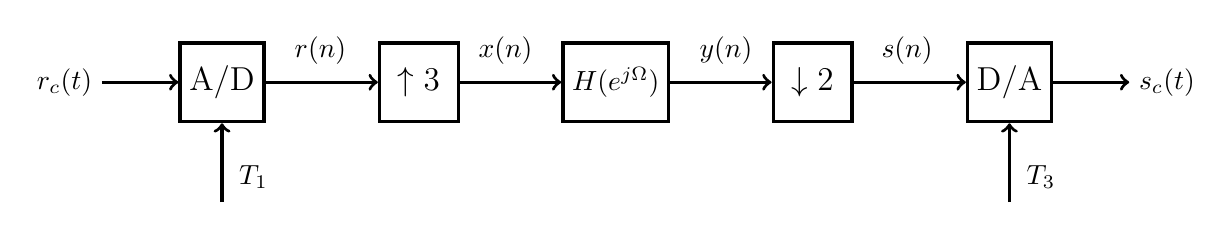
\begin{tikzpicture}[scale=1, transform shape]
    \node[rectangle, very thick, draw, minimum width=1cm, minimum height=1cm] (ad) at (0,0) {\large A/D};
    \node[rectangle, very thick, draw, minimum width=1cm, minimum height=1cm, xshift=2.5cm] (up) at (ad) {\large $\uparrow 3$};
    \node[rectangle, very thick, draw, minimum width=1cm, minimum height=1cm, xshift=2.5cm] (h) at (up) {$H(e^{j\Omega})$};
    \node[rectangle, very thick, draw, minimum width=1cm, minimum height=1cm, xshift=2.5cm] (down) at (h) {\large $\downarrow 2$};
    \node[rectangle, very thick, draw, minimum width=1cm, minimum height=1cm, xshift=2.5cm] (da) at (down) {\large D/A};

    \node[xshift=-2cm] (r_c) at (ad) {$r_c(t)$};
    \node[xshift=1.25cm,yshift=0.4cm] (r_n) at (ad) {$r(n)$};
    \node[xshift=1.1cm,yshift=0.4cm] (x_n) at (up) {$x(n)$};
    \node[xshift=1.4cm,yshift=0.4cm] (y_n) at (h) {$y(n)$};
    \node[xshift=1.2cm,yshift=0.4cm] (s_n) at (down) {$s(n)$};
    \node[xshift=2cm] (s_c) at (da) {$s_c(t)$};
    
    \node[yshift=-1.2cm,xshift=0.4cm] (t1) at (ad) {$T_1$};
    \node[yshift=-1.2cm,xshift=0.4cm] (t2) at (da) {$T_3$};

    \draw[->, very thick] (r_c.east) -- (ad.west);
    \draw[->, very thick] (ad.east) -- (up.west);
    \draw[->, very thick] (up.east) -- (h.west);
    \draw[->, very thick] (h.east) -- (down.west);
    \draw[->, very thick] (down.east) -- (da.west);
    \draw[->, very thick] (da.east) -- (s_c.west);
    \draw[->, very thick] (ad.south) ++ (0,-1cm) -- (ad.south) ;
    \draw[->, very thick] (da.south) ++ (0,-1cm) -- (da.south) ;
\end{tikzpicture}